\documentclass[sigconf]{acmart}

\usepackage{graphicx}
\usepackage{hyperref}
\usepackage{todonotes}

\usepackage{endfloat}
\renewcommand{\efloatseparator}{\mbox{}} % no new page between figures

\usepackage{booktabs} % For formal tables

\settopmatter{printacmref=false} % Removes citation information below abstract
\renewcommand\footnotetextcopyrightpermission[1]{} % removes footnote with conference information in first column
\pagestyle{plain} % removes running headers

\newcommand{\TODO}[1]{\todo[inline]{#1}}

\begin{document}
\title{Using Big Data For Fact Checking}

\author{Karthik Vegi}
\affiliation{%
  \institution{Indiana University Bloomington}
  \streetaddress{2619 East 2nd Street, Apt 11}
  \city{Bloomington, IN 47401} 
  \country{USA}}
\email{kvegi@iu.com}


% The default list of authors is too long for headers}
\renewcommand{\shortauthors}{kvegi}


\begin{abstract}
Big Data is no more the elephant in the room it once used to be. Since John Mashey coined the term in 1998, it has come a long way. It is often described as the three Vs: Volume, Velocity, and Variety of the data. Of late, a new dimension, \textit{Veracity} has been gaining importance which describes the quality and accuracy of the data. We show how Big Data can be used to spot fake news, bad data used by politicians, advertisers, and scientists.
\end{abstract}

\keywords{i523, hid231, big data, veracity, fact check, data accuracy}

\maketitle

\section{Introduction}

Big Data is playing a crucial role in building a smarter planet. Each and every action that we take leaves a digital footprint. Big Data is lending a great helping hand to crunch this data to make smarter decisions. ``Big Data is at the heart of the smart revolution. It is already completely transforming the way we live, find love, cure cancer, conduct science, improve performance, run cities and countries and operate business \cite{Marr2015}''  \\
``Large scale searches and analyses over multiple sources involves extracting data from highly heterogeneous structures, semantics, and qualities. One of the fundamental issues is that the extracted information can be biased, noisy, outdated, incorrect, misleading, and thus unreliable. To add to the problem, available data sources can provide conflicting information, leaving the users in doubt with respect to the accuracy \cite{Berti-Equille2016}.''  \\
``The impact of fake news on the recent election has focused public attention on this multi-tentacled and growing problem. Vast swaths of the population fall prey to such misinformation, while others struggle to discern unbiased truth from the morass of lies and distortions that surrounds us \cite{www-forbes2}.'' With so many data sources like media, internet, newspaper, and many more, it is not easy to spot fake news and fack check the data. We need to take the help of the technological advances like Big Data and Artificial Intelligence to handle this problem.\\ 
``Fake news and fact checking is clearly a data veracity problem. Veracity refers to several quality dimensions related to repairing data inconsistencies and fixing other data quality problems such as duplicates, missing or incomplete data. Data veracity can be attributed to the following: \\
\textbf{Ambiguity:} Data can be inconsistent from one source to another, leading to misinterpretation. \\
\textbf{Staleness:} The data is obsolete and no longer relevant. \\
\textbf{Falsification:} False or distorted information can be intentionally propagated by one source or a coalition of sources. Information can be manipulated or presented selectively to influence the audience and encourage and particular conclusion \cite{Berti-Equille2016}.'' 

\section{Fact Checking as a Big Data Problem}
Often veracity is not just about data quality, it is about data \textit{understandability}. But fake news is understandable and we can make great sense out of it by careful analysis. We should therefore strive to achieve \textit{truthfulness} \cite{www-forbes2}. ``Misinformation dynamics, in fact, is where the big data concept of data veracity and the problem of fake news connect. We are not simply talking about the accidental inaccuracies that make up the bulk of enterprise data quality efforts. On the contrary, fake news is intentional misinformation, and furthermore, it is dynamic \cite{www-forbes2}.''  \\
``A common strategy to evaluate the reliability of the sources is to take advantage of data redundancy, and rely on majority voting heuristic, which simply assigns a true label to data that are claimed by the majority of the sources. But this strategy is known to be error-prone, because it counts all the sources equally and does not consider source dependence \cite{www-forbes1}.'' \\ 
The social networking giants like Facebook and Twitter faced this problem and a lot of fingers were pointed at them for acting as a medium for spreading fake news. Facebook took the initiative to tackle the problem head on by implementing an option where the users can flag the story as false. The more false votes it garners, the less likely it is for it to appear on the news feed. It also displays a warning to the users mentioning that a lot of users have reported the story as false. But the problem here is that we are giving people a chance to alter truth. It also makes everyone believe that anything that is not flagged is true which might not always be the case \cite{www-forbes2} . \\ 
``To solve these problems, a combination of big data and AI methodologies are being developed that rely less on human-generated input, which can be swayed by opinion or a lack of facts. Google published a paper in 2015 about a new method of scoring web pages based on the accuracy of the facts presented. The algorithm assigns documents a trust score, which would then presumably be used as part of Google\textquotesingle s overall scoring to determine search rank. The technology is important, because it is attempting to understand a page\textquotesingle s context without the use of third-party signals, like links \cite{www-forbes1}.''  \\
``The news media and social media cannot be solely responsible for preventing fake news. Each one of us have equal responsibility to discern the accuracy. Tools already exist that can help individual users spot fake news sites. \textit{Hoaxy} is an online tool that helps people visualize the spread of claims and fact-checking online, and is available to anyone to use. Many Chrome extensions have been created that can alert and help filter fake news. Even popular websites like \textit{Snopes} and \textit{FactCheck.org} can help identify the most egregious fake stories \cite{www-forbes2}.''

\section{Big Data Techniques for fact checking}

\subsection{Recommendation Based Approaches}
Recommendation based approaches take the help of the community to determine the accuracy and quality of the sources. The reputation of the sources increases as more people agree that the source is reliable. These methods clearly have their shortcomings as people can be influenced by third party agencies to improve the trustworthiness of certain sources \cite{Berti-Equille2016}.

\subsection{Content Based Approaches}
``Content based approaches work by computing a trustworthiness score of a source as a function of the belief in its claims, and then the belief score of each claimed data as a function of trustworthiness of the sources asserting it \cite{Berti-Equille2016}.'' The source quality is initialized and iteratively updated based on the content belief. Various probabilistic methods have been used to tackle other aspects beyond trustworthiness and data belief \cite{Berti-Equille2016}. \\
In one such methodology, the truth discovery problem is transformed into a probabilistic inference model. An iterative algorithm is proposed which computes the posterior distribution of all the values of the sources and finds the one with the maximum probability. The model derives all the possible values reported by the sources and the conflicting values in the data streams and then calculates a score \cite{Zhao2014}. \\
\textbf{Figure 1} illustrates the content based approach for truth discovery in data streams. As there can be heterogeneous sources, first a semantic mapping is employed for the values provided by various sources, such that the values for truth discovery are consistent \cite{Zhao2014}. ``For example, the meaning of the weather conditions \textbf{\textit{rainy}} and \textbf{\textit{wet}} are considered to be the same in weather forecast truth discovery. Also \textbf{\textit{partly sunny}} and \textbf{\textit{mostly cloudy}} are grouped and considered to be the same as \textbf{\textit{clear}} \cite{Zhao2014}.'' \\
``At each time \textit{t}, the system collects a set of conflicting
values for entity \textit{i} as \textbf{\textit{V}} = $\left\{{v1,v2,...,vk}\right\}$ from multiple data sources. Next, the system resolves the conflicts and discovers the true value \textit{v} in \textit{V} based on the current data uncertainty and source
quality. Then, the system updates the data uncertainty and source quality based on the inferred value \textbf{v} and conflicting values \textit{V}. \cite{Zhao2014}''

\begin{figure}
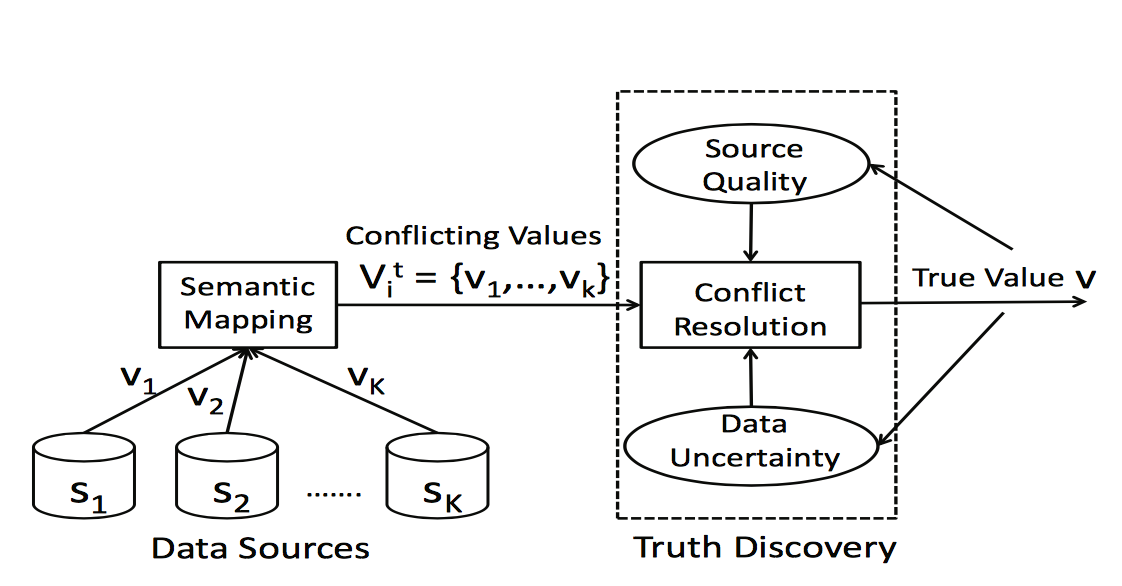
\includegraphics[width=0.7\textwidth]{images/fig1.png}
\caption{Truth Discovery In Data Streams \cite{Zhao2014}}
\end{figure}

\subsection{Evidence Based Approaches}
Evidence based approaches augment the content based approaches by relying on evidence, context and priori knowledge about the data sources \cite{Berti-Equille2016}. Data provenance information may be used in truth discovery computation, as well as external information about the context, the sources, the data or user network \cite{Berti-Equille2016}. This involves checking the dynamics of information in the network and recomputing the truth discovery accordingly \cite{Berti-Equille2016}. 
``The problem with evidence based practice is that outside of areas like health care and aviation is that most people in organizations do not care about having research evidence for almost anything they do. That does not mean they are not interesting in research but they are just not that interested in using the research to change how they do things \cite{www-oxford}''

\section{Automating Fact Checking}
In this digital age, fact checking makes more sense when it is done in real time. ``Politicians and media figures make claims about \textit{facts} all the time, but the new army of fact-checkers can often expose claims that are false, exaggerated or half-truths. The number of active fact-checking websites has grown from 44 a year ago to 64 in 2015, according the Duke Reporters’s Lab \cite{Hassan2015}.'' \\
The delay window between the time when a claim is made and the time when the claim is checked for truth has to be as less as possible. Fact checking takes longer time than traditional journalism. This gives enough time for the politicians and other people to make a claim and get away with it \cite{Hassan2015}

\subsection{Computational Challenges} 
\subsubsection{\textbf{Finding claims to check:}} This constitutes converting raw data to natural language and extracting contextual information such as speaker, time, and occasion \cite{Hassan2015}.
\subsubsection{\textbf{Getting data to check claims:}} This involves evaluating the quality and completeness of sources and mapping them back to the data sources. Integrating multiple sources and cleansing data is an integral part of this step \cite{Hassan2015}.

\subsection{Claimbuster}
\textbf{Claimbuster} is an online tool to check for facts in real time. ``For every sentence spoken by the participants of a presidential debate, Claimbuster determines whether the sentence has a factual claim and whether its truthfulness is important to the public. The calculation is based on machine learning models built from thousands of sentences from past debates labeled by humans. The ranking scores help journalists prioritize their efforts in assessing the veracity of claims. Claimbuster can be expanded to other discourses such as interviews and speeches and also adapted for use with social media \cite{Hassan2015}.'' \\
Claimbuster makes use of a supervised learning approach and breaks the sentences into three categories namely \textit{Non Factual Sentences}, \textit{Unimportant Factual Sentences}, and \textit{Check-worthy Factual Sentences} \cite{Hassan2015}. ``Given a sentence, the objective of Claimbuster is to derive a score that reflects the degree by which the sentence belongs to \textit{Check-worthy Factual Sentences}. Many widely-used classification methods support ranking naturally. For instance, consider a Support Vector Machine (SVM). \textit{Check-worthy Factual Sentences} are treated as positive examples and both \textit{Non Factual Sentences} and \textit{Unimportant Factual Sentences} as negative examples. SVM finds a decision boundary between the two types of training examples and calculates the posterior probability using a decision function. The probability scores of all sentences are used to rank them. This clearly will help the journalists and fact checkers to free up time to focus on more important things like reporting and writing \cite{Hassan2015}.''

\section{Conclusion}

Big Data coupled with Artificial Intelligence and Machine Learning can tackle the fact checking problem. Rather than working in silos, the social networking giants and the search engine giant could work together with researchers to come up with a more effective solution. This ensures that there are no loose ends with respect to the accuracy of the data. This is important because there is a disconnect between data sources at times and not everybody has control and access to data that somebody else owns.
    
\begin{acks}

The author would like to thank Dr. Gregor von Laszewski and the teaching assistants for their support and suggestions in writing this paper.

\end{acks}

\bibliographystyle{ACM-Reference-Format}
\bibliography{report} 



\section{Bibtex Issues}
\todo[inline]{Warning--empty chapter and pages in editor00}
\todo[inline]{(There was 1 warning)}
\section{Issues}
\end{document}
